\section*{Exercise 26.1-7}
\subsubsection*{Show that a flow network $G$ with vertex capacities can be transformed into a normal flow network $G'$. How many vertices and edges does $G'$ have?}
Let the $G$, $G'$, $v$ and $l$ be defined as in the exercise.

First we describes how a network $G_x$ where only one of the vertices, $x$, have a capacity constraint $l(x)$ and how it can be transformed into a new network without the vertex capacity constraint.

We define the set $E(x)$ of edges that have an edge going into the vertex with a capacity constraint. That is $E(x)  = \{(v,x) \in E: l(x)>0\}$.

To transform the network, we can augment $G_x$ with a new vertex $x'$ such that  $G_x' = (V',E')$ where $V' = V \cup \{x'\}$. We define $E'$ 
as $E' = E\setminus E(x) \cup E'(x) \cup \{(x',x)\}'$ where $E'(x)$ is the set of edges in $E(x)$, but with entrance point into the new vertex $x'$. So the set of edges $E'$ in the new transformed network consist of all edges in the original network, that did not have an edge going into the vertex with a capacity constraint. And all the edges that did go into the vertex with a capacity constraint have been replaced with new edges that goes into the new vertex $x'$. And a new edge have been introduced that goes from the new vertex $x'$ to the old vertex $x$. Hence in total one new vertex and one new edge have been introduced and none have been removed.

\begin{figure}[H]
\caption{\textit{Augmenting the network $G_x$ to $G_x'$}}
\vskip .2cm
\centering
\subfloat[Introducing the new vertex $x'$]{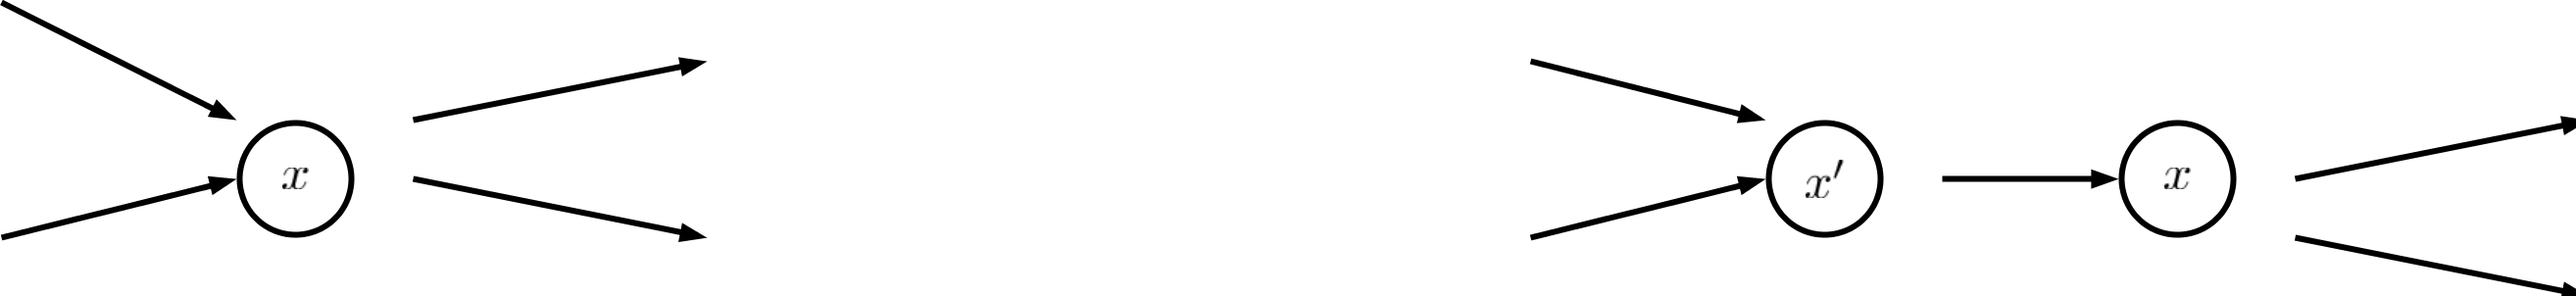
\includegraphics[angle=0,width=12cm]{26-1-7}}
\end{figure}

The capacity of the edges in the transformed network, where no vertex have a capacity is
\begin{align*}
c_{G_x'}(u,v) = 
\begin{cases}
c_{G_x}(u,x), & (u,v) = (u,x')\\
l(x), & (u,v) = (x',x)\\
c_{G_x}(u,v), & \text{else}
\end{cases}
\end{align*}
That is, the capacity for an edge going into $x'$ is the same as the capacity of going into $x$ in the $G_x$ network. The new edge have a capacity of $l(x)$ that is the capacity of the vertex in the $G_x$ network. In all other cases the capacity in the transformed network is the same as in the original network.

\begin{figure}[H]
\caption{\textit{Augmenting the network $G_x$ to $G_x'$}}
\vskip .2cm
\centering
\subfloat[Setting the edge capacities]{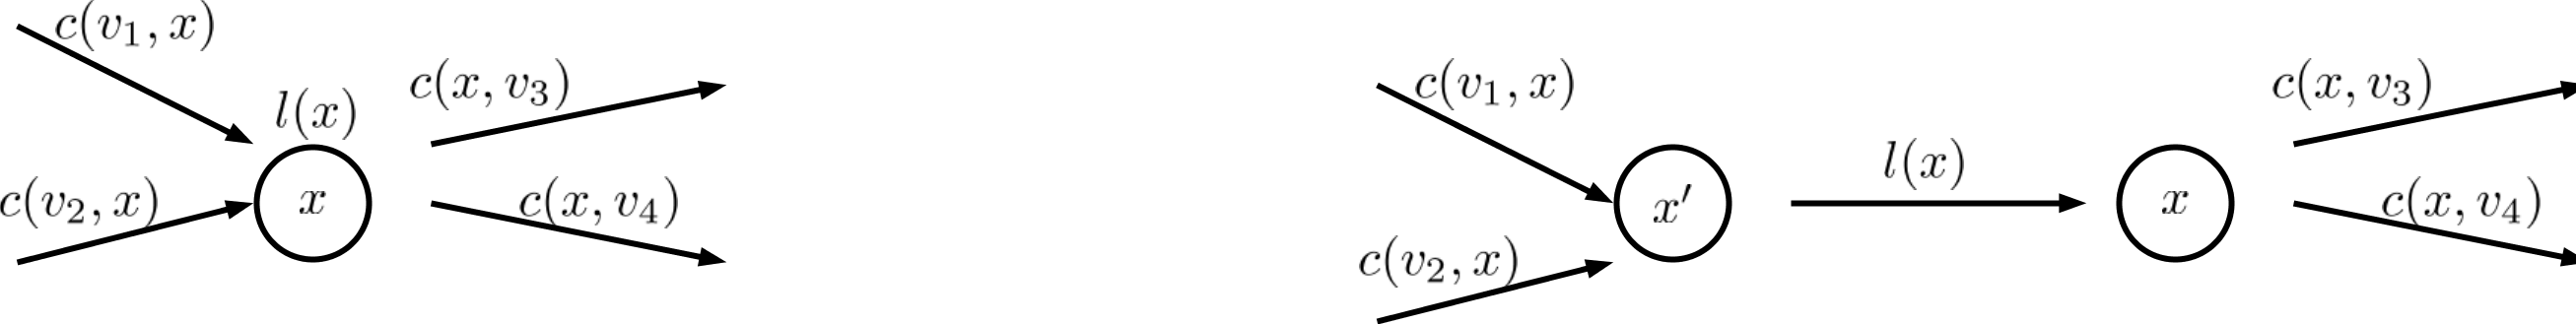
\includegraphics[angle=0,width=12cm]{26-1-7-withCapacity}}
\end{figure}

We have now shown how a network with a single vertex capacity constraint can be transformed into a new network without a capacity constraint. This can easily be generalized to an arbitrary number of vertex capacity constraint. If $x$ and $x'$ is replaced with $x_i$ and $x'_i$ in the above, all of what we have shown still holds, and for each vertex with a capacity constraint, there will be one new vertex and one new edge. Hence if all of the vertices, including the source and sink, had a constraint there would be $\abs{V}$ extra vertices and edges. So the total number of vertices in $G'$ would be $2\abs{V}$ and the total number of edges in $G'$ would be $\abs{E}+\abs{V}$.